\chapter{THIẾT KẾ HỆ THỐNG}\label{ch:thietke}

\section{Kiến trúc tổng thể và nguyên lý vận hành}
Hình~\ref{fig:kientruc} trình bày kiến trúc tổng thể được chuẩn hóa cho toàn bộ hệ thống. Cụm thiết bị đeo tại thắt lưng thu thập tín hiệu chuyển động và áp suất khí quyển, thực hiện xử lý trực tiếp trên vi điều khiển ESP32 rồi truyền trạng thái sang nút gắn trên mũ bảo hộ qua kết nối BLE. Tiếp theo, nút trên mũ bổ sung dữ liệu quan trắc môi trường và đóng gói bản tin tổng hợp để phát qua sóng vô tuyến RF 433 MHz. Ở phía thu, trạm chuyển tiếp Gateway sử dụng máy tính nhúng Raspberry Pi 3 Model B tiếp nhận gói tin, kiểm tra tính toàn vẹn, lưu vào hàng đợi đệm và đồng bộ lên máy chủ MQTT Broker thông qua mô-đun SIM 4G.

\Diagram{kien-truc}{Kiến trúc tổng thể của hệ thống với trạm chuyển tiếp Gateway Raspberry Pi 3B kết hợp mô-đun SIM 4G}{fig:kientruc}

Hình~\ref{fig:iot-tham-chieu} trình bày mô hình tham chiếu IoT bốn lớp theo khuyến nghị ITU-T Y.4000/Y.2060~\cite{itu}. Mô hình được dùng để đối chiếu chức năng của các khối trong kiến trúc đề tài, không thay thế sơ đồ kết nối thực tế ở Hình~\ref{fig:kientruc}.

\begin{figure}[htbp]
\centering
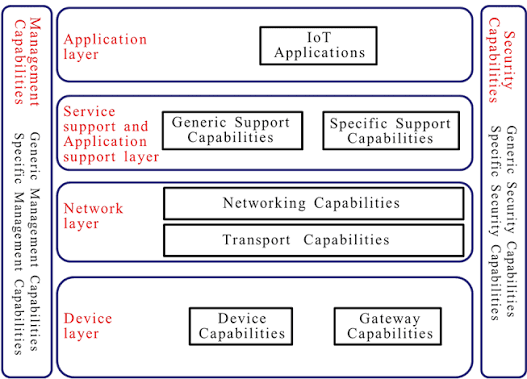
\includegraphics[width=.78\linewidth,height=.36\textheight,keepaspectratio]{assets/iot-architecture.png}
\caption{Mô hình tham chiếu IoT gồm bốn lớp chức năng cùng các năng lực quản lý và bảo mật xuyên suốt}
\label{fig:iot-tham-chieu}
\end{figure}

Trong cách đối chiếu này, \textit{lớp thiết bị} bao gồm cảm biến, nút ESP32 và Gateway; \textit{lớp mạng} bao gồm các chặng BLE, RF 433\,MHz và kết nối IP/4G; \textit{lớp hỗ trợ dịch vụ và ứng dụng} đảm nhận tiếp nhận, chuyển đổi, lưu đệm và phân phối bản tin qua MQTT Broker. \textit{Lớp ứng dụng} thể hiện mục tiêu khai thác thông tin trạng thái và cảnh báo phục vụ công tác chỉ huy, không đồng nghĩa với việc đã hoàn thành một ứng dụng phần mềm cụ thể. Hai nhóm năng lực quản lý và bảo mật áp dụng xuyên suốt cả bốn lớp, tương ứng với việc định danh thiết bị, giám sát liên kết, kiểm soát truy cập và bảo vệ dữ liệu.


Trong kiến trúc này, nút gắn trên mũ đóng vai trò là trạm tập trung dữ liệu trên cơ thể người lính. Cụm đeo thắt lưng và nút trên mũ được ghép nối theo cùng một mã định danh cá nhân. Tuy nhiên, dữ liệu chuyển động và dữ liệu môi trường vẫn giữ mã nguồn riêng biệt để hệ thống dễ dàng phát hiện trường hợp một trong hai mô-đun bị mất kết nối. Giao thức MQTT chỉ được triển khai trên chặng truyền dẫn có kết nối mạng IP từ trạm Gateway lên máy chủ. Vi điều khiển ESP32 chỉ truyền các khung dữ liệu ứng dụng dạng nhị phân qua BLE và sóng RF, hoàn toàn không đóng gói trực tiếp bản tin MQTT trên kênh vô tuyến 433 MHz.

Khi bắt đầu ca tác nghiệp, hệ thống tiến hành kiểm tra trạng thái cảm biến, khởi tạo tọa độ điểm xuất phát và thiết lập góc hướng chuẩn theo mặt bằng công trình. Trong suốt quá trình vận hành, các tiến trình đọc cảm biến, nhận dạng hoạt động, định vị quán tính và truyền thông được lập lịch thực thi độc lập. Khi một chặng kết nối bị gián đoạn, các phân hệ còn lại vẫn tiếp tục ghi nhận trạng thái và lưu dấu thời gian của bản tin hợp lệ cuối cùng. Giao diện giám sát trung tâm sẽ hiển thị rõ cảnh báo trễ dữ liệu này thay vì giữ nguyên giá trị cũ như thể hệ thống vẫn đang cập nhật bình thường.

\section{Thiết kế phần cứng thiết bị đeo}\label{sec:hardware}
\subsection{Cấu trúc linh kiện và chuẩn giao tiếp}
Khối thu thập chuyển động sử dụng mô-đun cảm biến quán tính GY-85 để đo gia tốc, vận tốc góc và từ trường trên cả ba trục tọa độ. Vi điều khiển trung tâm ESP32 trực tiếp đọc chuỗi dữ liệu thô, áp dụng tham số hiệu chuẩn và thực thi các thuật toán suy luận tại biên. Song song đó, cảm biến BMP580 cung cấp thông số áp suất khí quyển và nhiệt độ nội tại nhằm bổ sung ngữ cảnh môi trường và hỗ trợ phân tích độ biến thiên độ cao tương đối. Đặc tính đo áp suất và chuẩn giao tiếp số của cảm biến BMP580 được thiết lập theo đúng tài liệu kỹ thuật của nhà sản xuất Bosch~\cite{bmp580}.

\begin{figure}[htbp]\centering
\begin{subfigure}[t]{.46\linewidth}\centering
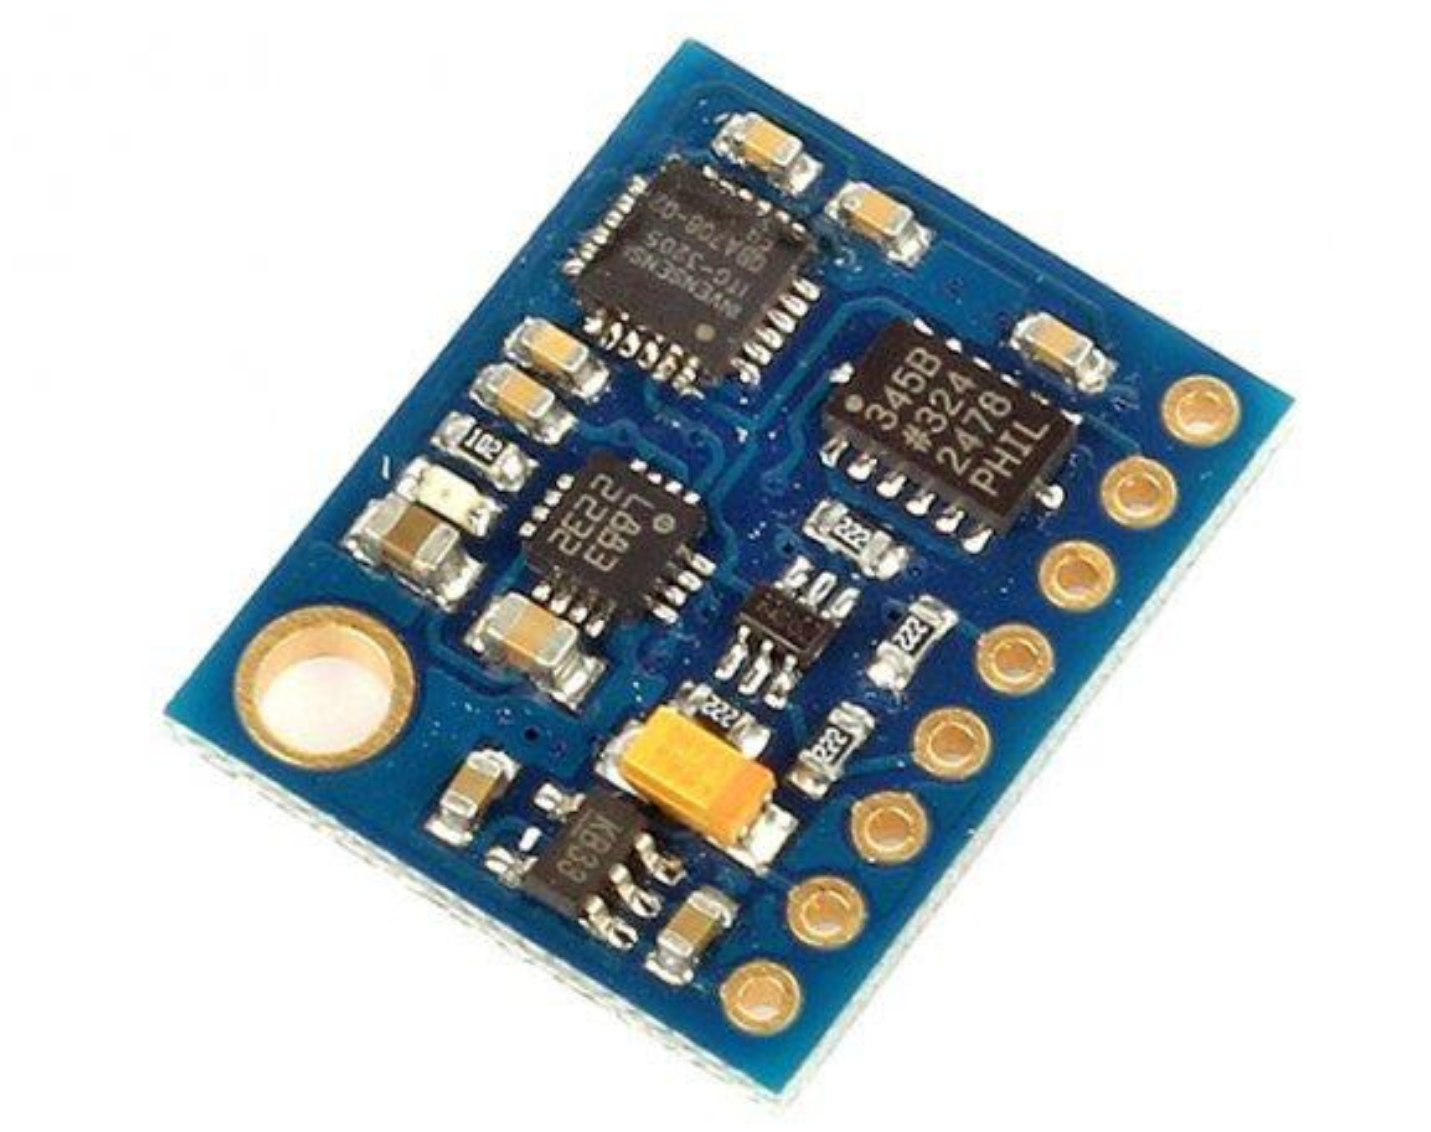
\includegraphics[width=.9\linewidth,height=5.5cm,keepaspectratio]{assets/gy85.png}
\caption{Mô-đun cảm biến quán tính GY-85}\end{subfigure}\hfill
\begin{subfigure}[t]{.46\linewidth}\centering
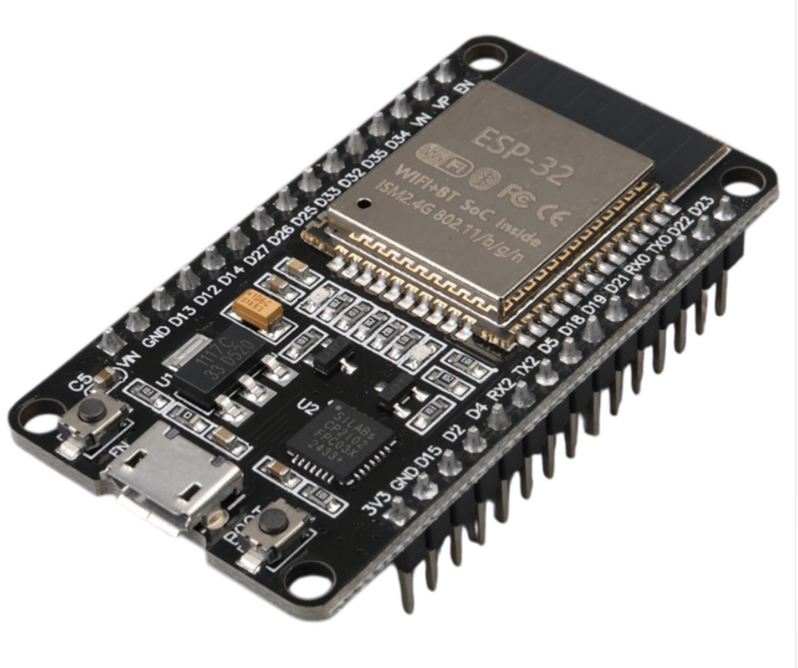
\includegraphics[width=.9\linewidth,height=5.5cm,keepaspectratio]{assets/esp32.png}
\caption{Bo mạch vi điều khiển ESP32}\end{subfigure}\par\vspace{10bp}
\begin{subfigure}[t]{.46\linewidth}\centering
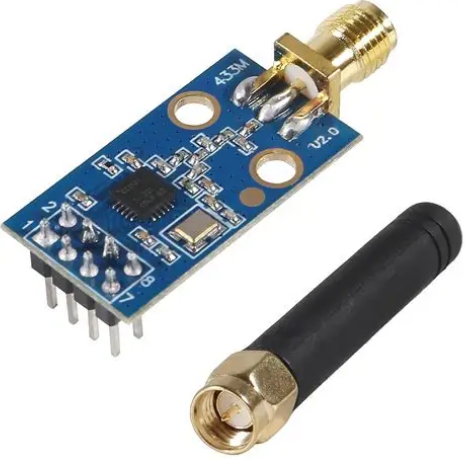
\includegraphics[width=.9\linewidth,height=5.5cm,keepaspectratio]{assets/rf433.png}
\caption{Mô-đun thu phát vô tuyến RF 433 MHz}\end{subfigure}\hfill
\begin{subfigure}[t]{.46\linewidth}\centering
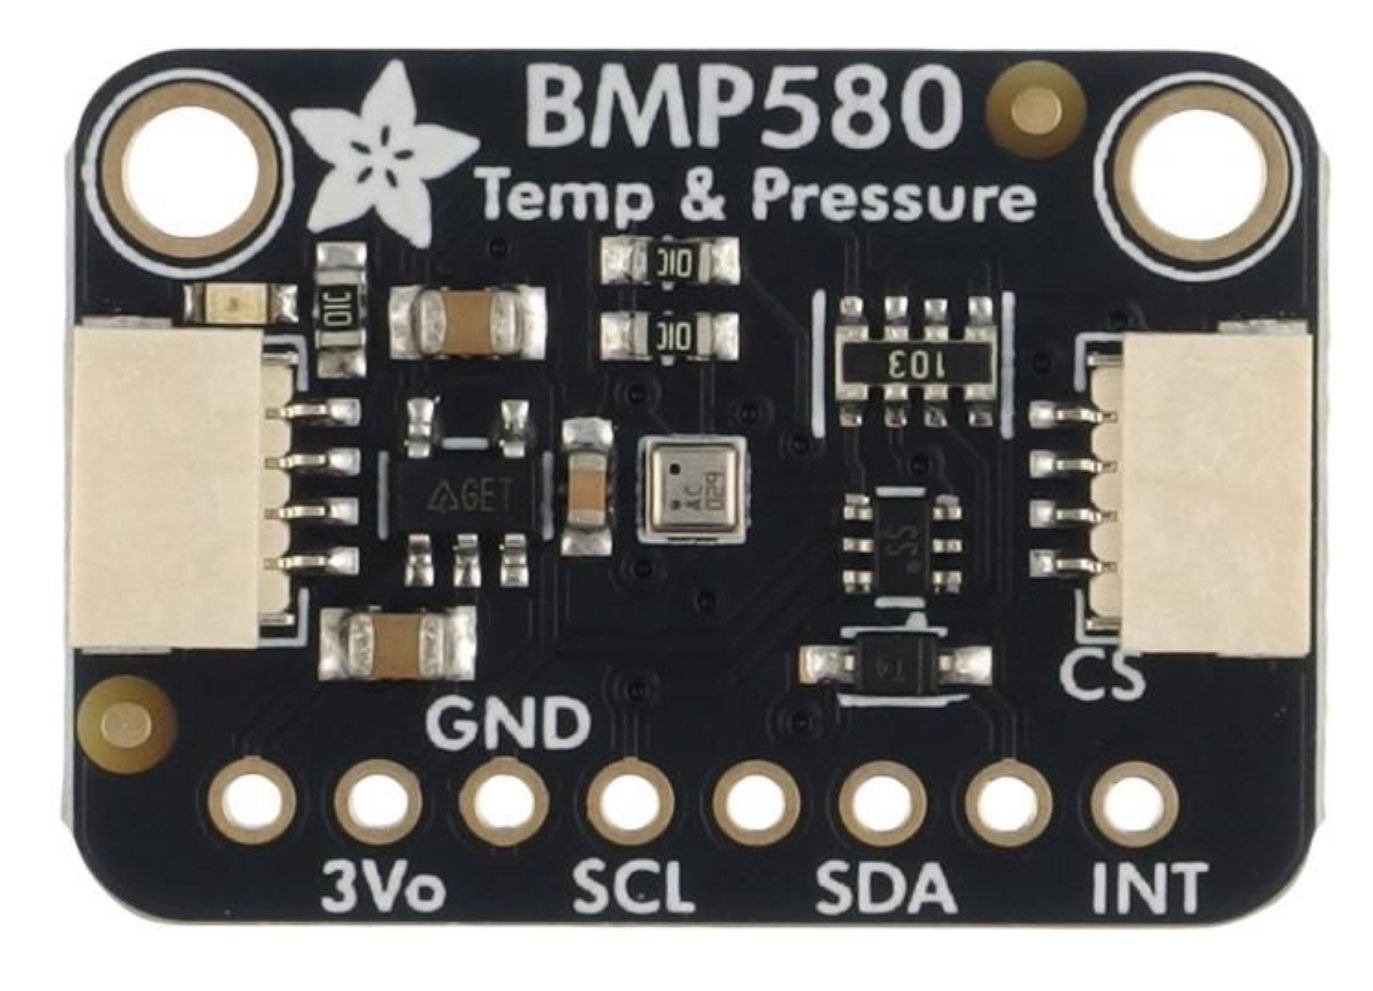
\includegraphics[width=.9\linewidth,height=5.5cm,keepaspectratio]{assets/bmp580.png}
\caption{Mô-đun cảm biến áp suất BMP580}\end{subfigure}
\caption{Các mô-đun phần cứng chính cấu thành hệ thống thiết bị đeo}
\label{fig:linhkien}
\SrcNote{Ảnh minh họa các thành phần phần cứng sử dụng trong hệ thống.}
\end{figure}

\begingroup\SmallTable
\begin{longtable}{|P{75bp}|P{115bp}|P{218bp}|}
\caption{Tổng hợp các chuẩn giao tiếp và điểm kiểm soát kỹ thuật phần cứng}\label{tab:hardware}\\\hline
\textbf{Khối phần cứng}&\textbf{Giao tiếp chức năng}&\textbf{Yêu cầu kiểm soát kỹ thuật}\\\hline\endfirsthead
\hline\textbf{Khối phần cứng}&\textbf{Giao tiếp chức năng}&\textbf{Yêu cầu kiểm soát kỹ thuật}\\\hline\endhead
Mô-đun GY-85&Giao tiếp I\textsuperscript{2}C với ESP32&Đối chiếu mã vi mạch, địa chỉ thanh ghi và chiều trục tọa độ thực tế; đọc dữ liệu thô, không giả định có sẵn thanh ghi góc phương vị tuyệt đối.\\\hline
Cảm biến BMP580&Giao tiếp I\textsuperscript{2}C với ESP32&Thiết lập địa chỉ không trùng lặp trên bus; đảm bảo khe thông khí cho cảm biến và cách ly nguồn nhiệt từ vi điều khiển.\\\hline
Vi điều khiển ESP32&Xử lý tại biên, BLE và quản lý nguồn&Tách biệt tiến trình lấy mẫu khỏi tác vụ truyền thông; giám sát sự kiện khởi động lại, số mẫu mất và dung lượng bộ đệm.\\\hline
Khối nguồn thiết bị đeo&Pin sạc, mạch bảo vệ và ổn áp&Đo kiểm độ sụt áp khi dòng tải biến thiên, kiểm tra dòng xung cực đại; gia cố dây dẫn và đầu nối chống đứt tuột cơ học.\\\hline
Nút tập trung trên mũ&Kết nối BLE, cảm biến khí và phát RF&Ghép nối đúng mã định danh thiết bị; quản lý tuổi dữ liệu; cách ly nhiệt và nhiễu dòng từ bộ đốt cảm biến khí khỏi khối IMU.\\\hline
Khối thu RF tại Gateway&Giao tiếp ngoại vi với Raspberry Pi 3B&Lựa chọn trình điều khiển đúng mã phần cứng thực tế. Đối với họ vi mạch CC1101, chuẩn giao tiếp điều khiển là SPI~\cite{cc1101}.\\\hline
\end{longtable}\endgroup

Trong cấu hình mô-đun GY-85 tham chiếu, vi mạch gia tốc kế ADXL345 hỗ trợ tùy chọn dải đo linh hoạt từ $\pm2g$ đến $\pm16g$~\cite{adxl345}. Khi thiết lập dải đo cho bài toán nhận dạng hoạt động và phát hiện té ngã, hệ thống cần cân bằng giữa độ phân giải tín hiệu và nguy cơ bão hòa biên độ khi va chạm mạnh. Cấu hình dải đo thực tế bắt buộc phải được ghi nhận rõ trong hồ sơ của từng phiên thu thập dữ liệu.

\subsection{Thiết kế nguồn cấp, đi dây và bố trí cơ khí}
Hệ thống nguồn trên bo mạch được phân tách độc lập thành nhánh cấp nguồn cho cảm biến, nhánh vi điều khiển và nhánh công suất phát vô tuyến. Cần phân biệt rõ mức điện áp đầu vào nuôi bo mạch phát triển với mức điện áp logic trên các chân tín hiệu. Vi điều khiển ESP32 hoạt động ở mức điện áp logic chuẩn 3,3 V theo quy định trong tài liệu kỹ thuật~\cite{esp32}. Do đó, mọi tín hiệu điện áp từ các mô-đun ngoại vi đều phải được kiểm tra tương thích mức logic trước khi kết nối vào chân GPIO hoặc bộ chuyển đổi ADC.

Đối với các cảm biến khí bán dẫn có phần tử đốt nóng nội tại và ngõ ra điện áp tương tự, mạch giao tiếp cần được tính toán cầu phân áp hoặc bổ sung tầng khuếch đại đệm phù hợp. Việc cấu hình hệ số suy hao ADC bằng phần mềm hoàn toàn không giúp chân vi điều khiển chịu được mức điện áp vượt ngưỡng phần cứng cho phép. Độ ổn định của đường nguồn và mặt phẳng nối đất (mass) cần được đo kiểm kỹ trong điều kiện bộ phát RF, bộ đốt cảm biến khí và vi điều khiển hoạt động đồng thời ở công suất tối đa.

Về mặt cơ khí, mô-đun GY-85 phải được cố định chắc chắn vào khung vỏ, đánh dấu rõ chiều trục tọa độ và giữ nguyên vị trí xuyên suốt từ giai đoạn thu thập dữ liệu huấn luyện đến khi vận hành thực tế. Vị trí đeo thiết bị tại vùng thắt lưng cần được chuẩn hóa nhất quán. Do các đường mạch mang dòng điện lớn, cuộn cảm nguồn xung và vật liệu sắt từ dễ làm méo từ trường cục bộ, quá trình hiệu chuẩn từ kế bắt buộc phải thực hiện sau khi đã lắp ráp hoàn chỉnh cả pin, ăng-ten và vỏ hộp, thay vì chỉ hiệu chuẩn trên bo mạch rời.

Cảm biến áp suất BMP580 cần được bố trí khe thông khí hợp lý trên vỏ hộp; việc đóng kín hoàn toàn hoặc làm che khuất lỗ thông hơi sẽ gây trễ pha đáp ứng áp suất. Ngoài ra, cảm biến nhiệt độ tích hợp bên trong BMP580 chịu ảnh hưởng trực tiếp từ nhiệt lượng tỏa ra của bo mạch điện tử. Vì vậy, hệ thống chỉ sử dụng thông số này để bù nhiệt cho phép đo áp suất nội bộ, không dùng để kết luận nhiệt độ môi trường không khí bên ngoài nếu chưa có cơ chế cách ly nhiệt.


\subsection{Sơ đồ nguyên lý và mô hình PCB thử nghiệm}\label{subsec:pcb-minhchung}
Sơ đồ nguyên lý ở Hình~\ref{fig:pcb-schematic} là tài liệu thiết kế bo mạch thử nghiệm kết hợp vi điều khiển ESP32-C5 với mô-đun GY-85. Bản vẽ thể hiện các khối đầu vào USB Type-C, quản lý nguồn dùng IP5306, ổn áp AMS1117-3.3V, giao tiếp cảm biến GY-85 qua I\textsuperscript{2}C, đầu đọc thẻ nhớ, các nút nhấn và đèn báo trạng thái. Các đường tín hiệu \texttt{SDA}, \texttt{SCL}, \texttt{IMU\_INT} được dẫn về vi điều khiển; nguồn logic được ký hiệu \texttt{3V3}. Mã mô-đun tại vị trí U4 của bản vẽ là \texttt{ESP32-C5-WROOM-1-N16R8-V1.2}.

\begin{figure}[htbp]
  \centering
  \IfFileExists{assets/schematic-gy85-esp32c5.pdf}{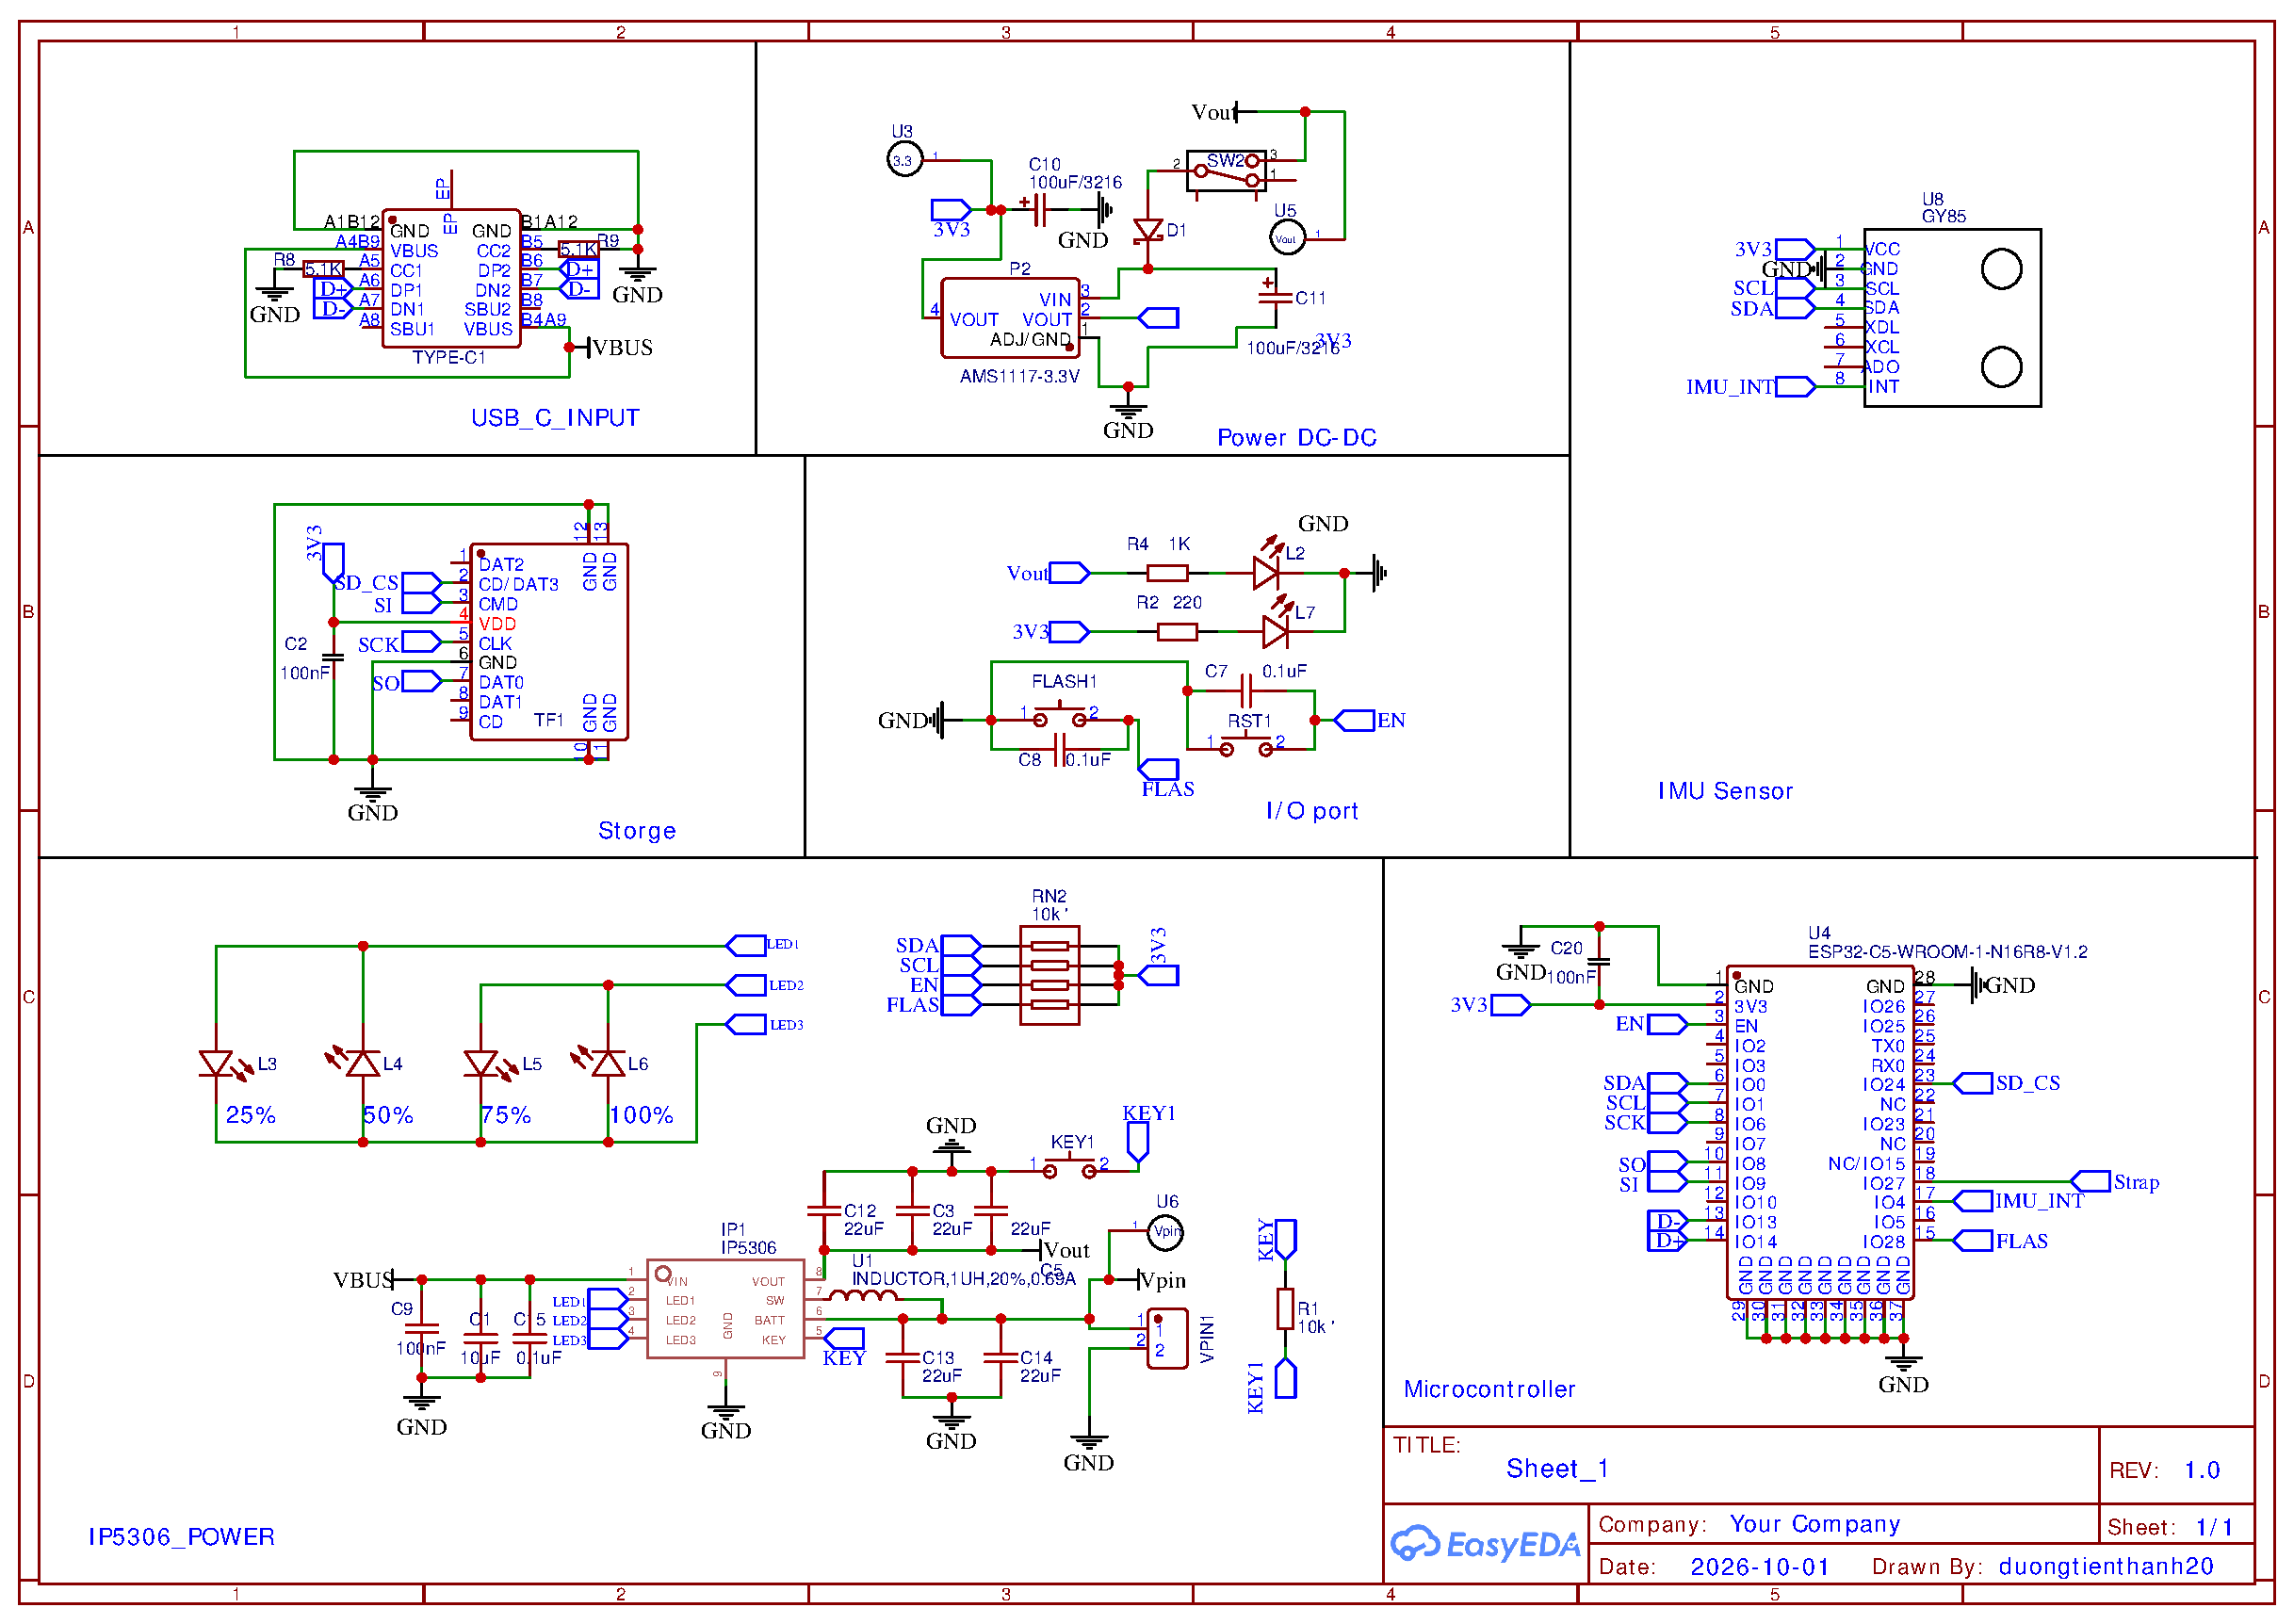
\includegraphics[width=\linewidth,height=.66\textheight,keepaspectratio]{assets/schematic-gy85-esp32c5.pdf}}{\fbox{\parbox{.82\linewidth}{Tư liệu PDF sơ đồ nguyên lý được cung cấp trong gói ảnh của báo cáo.}}}
  \caption{Sơ đồ nguyên lý bo mạch thử nghiệm sử dụng ESP32-C5 và GY-85}
  \label{fig:pcb-schematic}
\end{figure}

Hình~\ref{fig:pcb-3d-tren} và Hình~\ref{fig:pcb-3d-duoi} thể hiện mô hình ba chiều của hai mặt bo mạch. Các hình ảnh cho phép quan sát vị trí lắp mô-đun ESP32-C5, cụm nút nhấn, đầu nối, ổn áp, linh kiện nguồn và khe thẻ nhớ trước bước chế tạo. Đây là hình mô phỏng bố trí linh kiện PCB, không phải kết quả đo điện áp, kiểm tra đường mạch hay ảnh chụp thiết bị đã lắp ráp thực tế.

\begin{figure}[htbp]
  \centering
  \IfFileExists{assets/pcb-3d-mat-tren.png}{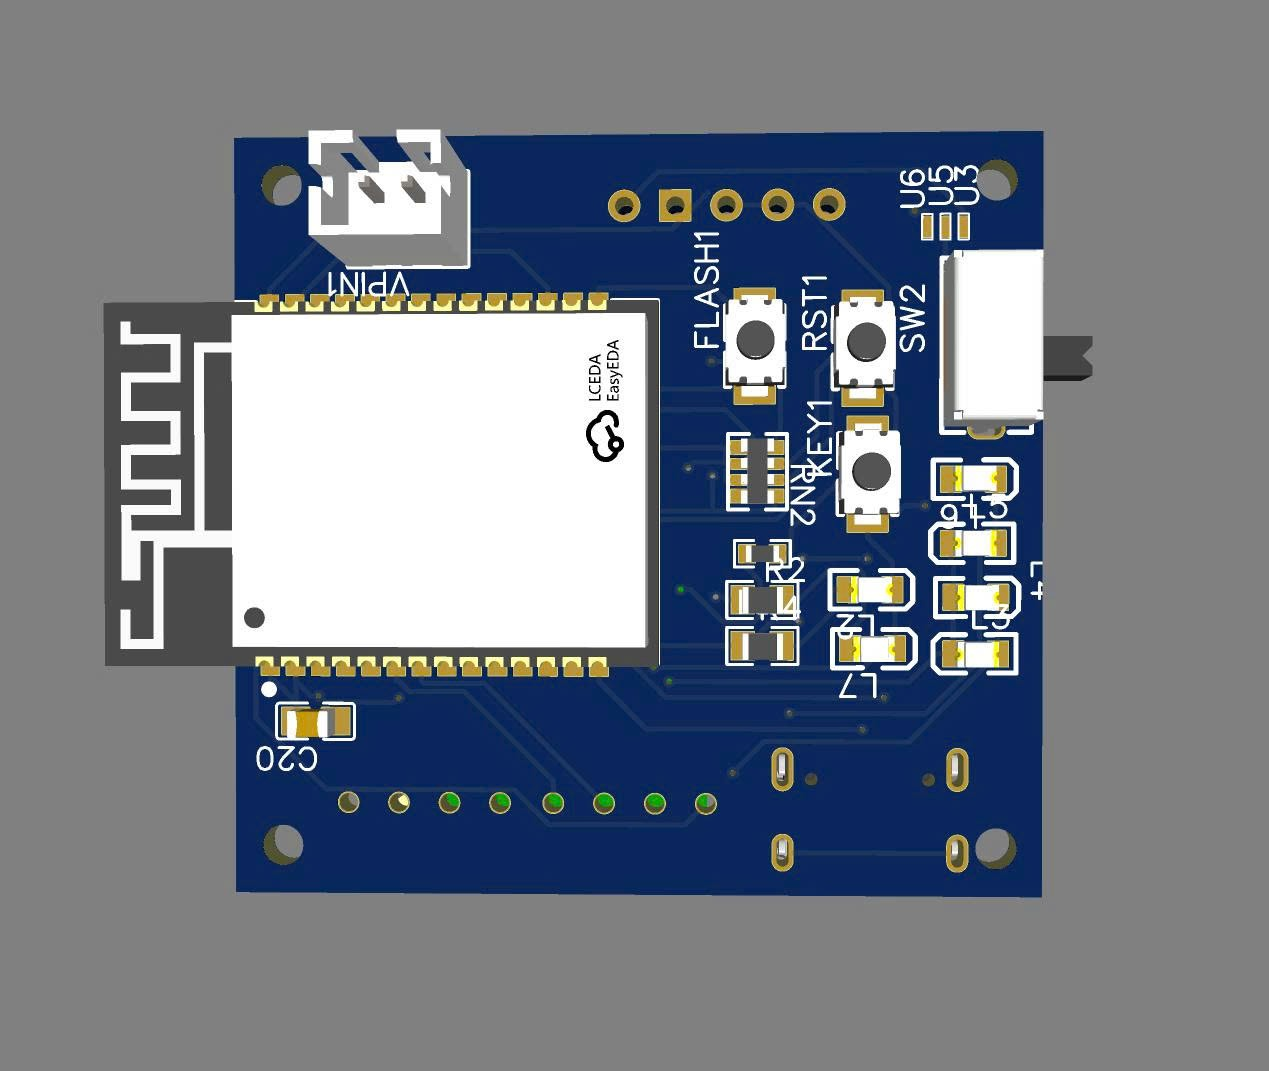
\includegraphics[width=.82\linewidth,height=.43\textheight,keepaspectratio]{assets/pcb-3d-mat-tren.png}}{\fbox{\parbox{.82\linewidth}{Ảnh mô hình 3D mặt bo mạch có mô-đun ESP32-C5 và các nút nhấn.}}}
  \caption{Mô hình 3D một mặt bo mạch thử nghiệm với mô-đun ESP32-C5 và cụm nút nhấn}
  \label{fig:pcb-3d-tren}
\end{figure}

\begin{figure}[htbp]
  \centering
  \IfFileExists{assets/pcb-3d-mat-duoi.png}{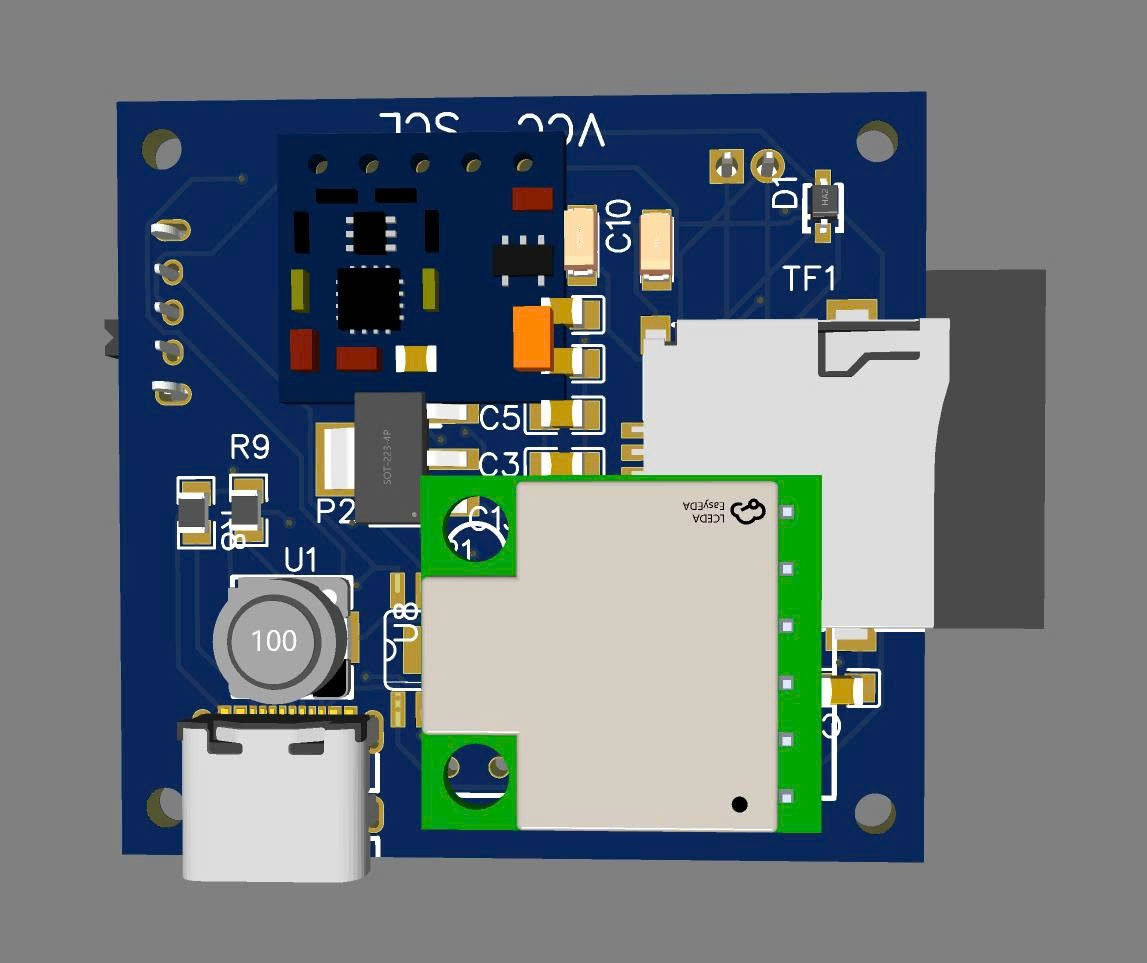
\includegraphics[width=.82\linewidth,height=.43\textheight,keepaspectratio]{assets/pcb-3d-mat-duoi.png}}{\fbox{\parbox{.82\linewidth}{Ảnh mô hình 3D mặt bo mạch có khối nguồn và khe thẻ nhớ.}}}
  \caption{Mô hình 3D mặt còn lại của bo mạch, thể hiện khối nguồn và khe thẻ nhớ}
  \label{fig:pcb-3d-duoi}
\end{figure}

Sơ đồ này phản ánh riêng bo mạch thử nghiệm ESP32-C5--GY-85; các phần tử RF 433 MHz, mô-đun SIM 4G, Raspberry Pi 3B và cảm biến BMP580 trong kiến trúc tổng thể được mô tả ở các phần riêng. Do đó, hình nguyên lý không được xem là bằng chứng tất cả các khối của hệ thống hoàn chỉnh đã được tích hợp lên cùng một PCB.

\section{Thiết kế trạm chuyển tiếp Gateway Raspberry Pi 3B kết hợp mô-đun SIM 4G}\label{sec:gateway}
\subsection{Cấu hình phần cứng và phân bổ tác vụ xử lý}
Trạm chuyển tiếp Gateway sử dụng máy tính nhúng Raspberry Pi 3 Model B trang bị vi xử lý bốn nhân BCM2837 tốc độ 1,2 GHz, bộ nhớ RAM 1 GB cùng các giao tiếp USB 2.0, Ethernet và GPIO~\cite{pi}. Trong kiến trúc hệ thống, Raspberry Pi 3B đảm nhận vai trò thu nhận gói tin từ khối vô tuyến RF, vận hành dịch vụ chuyển tiếp và quản lý hàng đợi dữ liệu. Mô-đun SIM 4G kết nối với Raspberry Pi 3B giúp thiết lập giao diện mạng IP di động, trong đó thẻ SIM và cấu hình điểm truy cập (APN) được thiết lập tương thích với nhà mạng viễn thông.

Toàn bộ tác vụ xử lý tín hiệu chuyển động và suy luận học máy vẫn được thực thi hoàn toàn tại biên trên vi điều khiển ESP32. Trạm Gateway không cần thu nhận liên tục chuỗi dữ liệu cảm biến thô để tính toán lại từ đầu. Thay vào đó, Raspberry Pi 3B tập trung kiểm tra tính toàn vẹn của bản tin, gắn dấu thời gian tiếp nhận, lưu trữ vào bộ đệm an toàn, chuyển đổi khung nhị phân sang định dạng bản tin cấu trúc và duy trì kết nối ổn định với MQTT Broker. Cách phân bổ tác vụ này giúp quá trình lấy mẫu thời gian thực trên thiết bị đeo hoàn toàn độc lập với sự biến động băng thông của mạng di động 4G.

\subsection{Chuỗi phần cứng thu phát và quy trình thiết lập kết nối}
Ở phía thu vô tuyến, trạm Gateway cần trang bị mô-đun thu RF tương thích hoàn toàn về tần số sóng mang, phương thức điều chế và cấu trúc gói tin với nút phát trên mũ bảo hộ. Nếu sử dụng mô-đun thu phát thuộc họ vi mạch CC1101, khối RF sẽ giao tiếp trực tiếp với Raspberry Pi 3B qua chuẩn SPI; trường hợp sử dụng mô-đun thu tích hợp sẵn vi điều khiển giải mã trung gian, chuẩn giao tiếp đầu vào có thể là UART hoặc USB~\cite{cc1101}. Việc lựa chọn trình điều khiển phần mềm và sơ đồ đấu nối phải căn cứ vào mã vi mạch thực tế trên bo mạch, không suy diễn chủ quan chỉ từ nhãn tần số ``433 MHz''.

Ở phía kết nối mạng diện rộng, quy trình tích hợp mô-đun SIM 4G trên hệ điều hành Linux diễn ra tuần tự qua các bước: nhận diện thiết bị phần cứng, kiểm tra trạng thái thẻ SIM, khai báo tham số APN, khởi tạo giao diện mạng IP, kiểm tra bảng định tuyến cùng dịch vụ phân giải tên miền (DNS), và cuối cùng là thiết lập phiên kết nối tới MQTT Broker. Việc mô-đun SIM 4G báo có sóng di động hoặc đọc được mã SIM chưa đủ cơ sở để khẳng định dữ liệu đã truyền tới máy chủ thành công. Toàn bộ các chặng truyền dẫn đều phải ghi nhận nhật ký hoạt động kèm mã định danh gói tin để phục vụ kiểm tra đối chứng.

Ngân sách nguồn cấp cho trạm Gateway phải được tính toán tổng thể cho cả bo mạch Raspberry Pi 3B, mô-đun thu RF và mô-đun SIM 4G. Tài liệu kỹ thuật của Raspberry Pi khuyến nghị sử dụng bộ nguồn chuẩn 5 V -- 2,5 A cho riêng bo mạch Pi 3B~\cite{pipower}. Do mô-đun SIM 4G thường tiêu thụ dòng điện xung rất lớn khi phát sóng ở khu vực sóng yếu, hệ thống cần kiểm tra kỹ hiện tượng sụt áp trên cáp dẫn và giới hạn cấp dòng của cổng giao tiếp. Thiết kế cần bố trí nhánh cấp nguồn độc lập có dòng tải đủ lớn cho mô-đun SIM 4G.

\subsection{Cơ chế quản lý hàng đợi và giám sát trạng thái kết nối}
Hình~\ref{fig:gateway} minh họa luồng xử lý hàng đợi và chuyển tiếp bản tin của trạm Gateway qua kết nối SIM 4G. Ngay khi nhận được khung tin RF hợp lệ, hệ thống lập tức ghi bản tin vào hàng đợi lưu trữ bền vững trên thẻ nhớ trước khi thực hiện truyền mạng. Một khóa định danh duy nhất kết hợp giữa mã thiết bị, mã phiên khởi động và số thứ tự gói tin được thiết lập nhằm loại bỏ các bản tin trùng lặp khi mạng RF hoặc giao thức MQTT thực hiện phát lại. Các gói tin lưu đệm vẫn bảo toàn dấu thời gian gốc tại thời điểm đo trên thiết bị đeo, đồng thời được gắn thêm dấu thời gian tiếp nhận tại Gateway để phần mềm giám sát phân biệt rõ dữ liệu thời gian thực với dữ liệu đồng bộ bù sau khi khôi phục mạng.

\Diagram{gateway}{Luồng quản lý hàng đợi lưu đệm và chuyển tiếp dữ liệu trên trạm Gateway Raspberry Pi 3B}{fig:gateway}

Bộ nhớ hàng đợi trên Gateway được thiết lập giới hạn dung lượng tối đa đi kèm chính sách giải phóng bộ nhớ rõ ràng. Trong đó, các bản tin sự kiện cảnh báo khẩn cấp luôn được gán quyền ưu tiên cao nhất; các gói tin trạng thái định kỳ có thể được nén gộp hoặc giới hạn thời gian lưu trữ nhằm tránh làm tràn bộ nhớ khi mất kết nối 4G kéo dài. Trạm Gateway chỉ đánh dấu hoàn tất chuyển giao bản tin sau khi nhận được gói tin xác nhận phản hồi từ máy chủ MQTT Broker. Cần lưu ý rằng tín hiệu xác nhận ở tầng MQTT chỉ đảm bảo dữ liệu đã tới Broker, việc kiểm tra hiển thị chính xác trên giao diện người dùng là một quy trình nghiệm thu độc lập.

Bên cạnh đó, trạm Gateway liên tục giám sát các trạng thái lỗi bao gồm mất tín hiệu RF từ mũ bảo hộ, đứt kết nối BLE cục bộ (được báo cáo trong cờ trạng thái từ mũ), lỗi mô-đun SIM 4G và khoảng thời gian trôi qua kể từ gói tin hợp lệ cuối cùng. Cơ chế giám sát đa tầng này giúp giao diện chỉ huy phân biệt chính xác nguyên nhân sự cố đến từ hỏng hóc cảm biến, mất liên kết trên cơ thể người lính hay gián đoạn đường truyền mạng diện rộng.

\section{Tổ chức cấu trúc dữ liệu và giao thức tầng ứng dụng}\label{sec:data}
\subsection{Thiết kế khung bản tin nhị phân trên đường truyền RF}
Để tối ưu hóa băng thông và giảm thời gian chiếm kênh trên đường truyền vô tuyến 433 MHz, dữ liệu được đóng gói dưới dạng khung nhị phân kích thước cố định thay vì truyền chuỗi văn bản JSON dung lượng lớn. Bảng~\ref{tab:frame} trình bày chi tiết cấu trúc khung bản tin ứng dụng 44 byte được thiết kế cho hệ thống. Để giải mã chính xác, chương trình nhúng ở cả đầu phát và đầu thu phải thống nhất tuyệt đối về phiên bản lược đồ, thứ tự sắp xếp byte (endianness) và hệ số quy đổi đơn vị vật lý.

\begingroup\SmallTable
\begin{longtable}{|P{114bp}|P{35bp}|P{259bp}|}
\caption{Cấu trúc khung bản tin ứng dụng nhị phân 44 byte trên đường truyền RF}\label{tab:frame}\\\hline
\textbf{Trường dữ liệu}&\textbf{Số byte}&\textbf{Mô tả ý nghĩa và quy ước định dạng}\\\hline\endfirsthead
\hline\textbf{Trường dữ liệu}&\textbf{Số byte}&\textbf{Mô tả ý nghĩa và quy ước định dạng}\\\hline\endhead
Phiên bản và loại bản tin&2&Gồm hai trường 1 byte; định danh phiên bản giao thức và phân biệt gói tin định kỳ với gói sự kiện khẩn cấp.\\\hline
Mã định danh thiết bị&2&Mã số định danh duy nhất của cụm thiết bị đeo hoặc chiến sĩ trong ca tác nghiệp.\\\hline
Mã phiên khởi động&2&Phân biệt các chuỗi đếm số thứ tự khác nhau sau mỗi lần thiết bị khởi động lại.\\\hline
Số thứ tự gói tin&4&Bộ đếm gói tin tăng đơn điệu, dùng để phát hiện mất gói và lọc bỏ bản tin trùng lặp.\\\hline
Dấu thời gian thiết bị&4&Thời gian hoạt động tính bằng mili-giây (ms) từ lúc khởi động; có kiểm soát tràn bộ đếm.\\\hline
Tổng số bước chân&4&Tổng số bước chân cộng dồn tính từ thời điểm khởi tạo phiên định vị.\\\hline
Tọa độ tương đối $x,y$&8&Mỗi trục tọa độ gồm 4 byte có dấu, biểu diễn theo đơn vị cm so với điểm gốc xuất phát.\\\hline
Góc phương vị&2&Giá trị góc hướng di chuyển tính theo đơn vị $0{,}01^\circ$ theo hệ quy chiếu chuẩn.\\\hline
Áp suất khí quyển&4&Giá trị áp suất đo được từ cảm biến, biểu diễn theo đơn vị Pascal (Pa).\\\hline
Nhãn hành động và độ tin cậy&2&Gồm hai trường 1 byte; chứa mã phân loại hoạt động (0--10) và điểm tin cậy đã chuẩn hóa.\\\hline
Điện áp nguồn pin&2&Biểu diễn theo đơn vị mili-vôn (mV); cần hiệu chuẩn hệ số cầu phân áp đo pin.\\\hline
Dữ liệu thô cảm biến khí&4&Mỗi cảm biến khí chiếm 2 byte lưu giá trị ADC hoặc điện trở thô; không mặc định là nồng độ PPM chuẩn.\\\hline
Cờ báo trạng thái hệ thống&2&Các bit trạng thái phản ánh tính hợp lệ của cảm biến, kết nối BLE, chất lượng góc hướng và mã lỗi.\\\hline
Mã kiểm tra lỗi CRC&2&Mã kiểm tra độ toàn vẹn của khung tin ứng dụng; không đóng vai trò là mã xác thực bảo mật.\\\hline
\textbf{Tổng kích thước}&\textbf{44}&Kích thước tải ứng dụng, chưa bao gồm phần tiền tố (preamble) và đồng bộ của lớp vật lý vô tuyến.\\\hline
\end{longtable}\endgroup

Khi mở rộng hệ thống cho nhiều chiến sĩ hoạt động đồng thời, tốc độ bit hữu ích ở tầng ứng dụng được ước tính theo công thức $R=N \cdot f \cdot B \cdot 8$, trong đó $N$ là số lượng nút mạng, $f$ là tần suất phát gói tin mỗi giây và $B$ là kích thước byte của khung ứng dụng. Ví dụ, với cấu hình 4 thiết bị cùng phát 1 gói tin 44 byte mỗi giây, tốc độ dữ liệu hữu ích tạo ra là 1.408 bit/s. Cần lưu ý rằng đây chỉ là phép tính dung lượng tải thuần túy ở tầng ứng dụng, chưa bao gồm các byte tiền tố phần cứng, gói tin xác nhận, thời gian phát lại và độ trễ do tranh chấp kênh truyền vô tuyến; do đó không sử dụng con số này như kết quả đo thông lượng thực tế hay cam kết về vùng phủ sóng.

\subsection{Quy hoạch cấu trúc chủ đề MQTT và kiểm soát trùng lặp}
Khi dữ liệu được đẩy lên máy chủ MQTT Broker, các luồng bản tin được phân nhánh rõ ràng theo mã nhiệm vụ và mã định danh thiết bị, ví dụ: \nolinkurl{firefighter/mission01/node01/telemetry} cho dữ liệu định kỳ, \texttt{.../event} cho cảnh báo khẩn cấp và \texttt{.../status} cho trạng thái phần cứng. Trong quá trình chuyển đổi từ khung nhị phân RF sang gói tin cấu trúc MQTT, trạm Gateway giữ nguyên số thứ tự gói và dấu thời gian gốc của thiết bị đeo, đồng thời chèn thêm dấu thời gian tiếp nhận tại Gateway, trạng thái kết nối, đơn vị đo và phiên bản lược đồ dữ liệu.

Cơ chế lọc chống trùng lặp gói tin được thiết lập chặt chẽ trong phạm vi từng nhiệm vụ và từng phiên khởi động thiết bị. Cách tổ chức này giúp hệ thống tránh được lỗi loại bỏ nhầm các gói tin mới có số thứ tự quay về 0 sau khi thiết bị đeo bị khởi động lại. Ngoài ra, khoảng thời gian mất kết nối, thời điểm nhận dữ liệu bù và cờ báo dữ liệu quá hạn đều được tách thành các trường thông tin độc lập để phần mềm giám sát không vẽ nối các tọa độ lịch sử như một chuyển động vừa mới diễn ra.

\section{Thiết kế mô hình nhận dạng hành động tại biên trên ESP32}\label{sec:har}
\subsection{Phân đoạn cửa sổ dữ liệu và cấu hình mô hình học máy}
Hệ thống thu thập tín hiệu gia tốc với tần số lấy mẫu $f_s=50$ Hz và phân đoạn thành các cửa sổ thời gian cố định có độ dài $T=3$ giây, tương ứng với số mẫu dữ liệu trong mỗi cửa sổ là:
\begin{equation}
N=f_sT=150\ \text{mẫu trên mỗi trục tọa độ}.
\end{equation}
Mô hình phân loại sử dụng thuật toán Rừng ngẫu nhiên (Random Forest) gồm 17 cây quyết định, giới hạn độ sâu tối đa 14 tầng với véc-tơ đầu vào gồm 13 đặc trưng thống kê. Toàn bộ dung lượng bộ nhớ Flash, mức chiếm dụng RAM và thời gian suy luận của mô hình đều được đặt trong mối tương quan đánh giá chung khi chạy đa nhiệm cùng tiến trình lấy mẫu và truyền thông trên vi điều khiển ESP32 (Hình~\ref{fig:har}).

\Diagram{har}{Sơ đồ phân tách giai đoạn huấn luyện mô hình ngoại tuyến và giai đoạn suy luận thời gian thực trên ESP32}{fig:har}

Hình~\ref{fig:har-quy-trinh-minh-hoa} minh họa chuỗi công việc từ thu thập dữ liệu 11 trạng thái hoạt động của lính cứu hỏa, theo dõi biến thiên tín hiệu trong cửa sổ thời gian đến trích chọn đặc trưng và suy luận trên vi điều khiển. Đây là hình diễn giải nguyên lý xử lý; hình không thay thế số liệu đánh giá độ chính xác hoặc độ trễ của mô hình.

\begin{figure}[htbp]
\centering
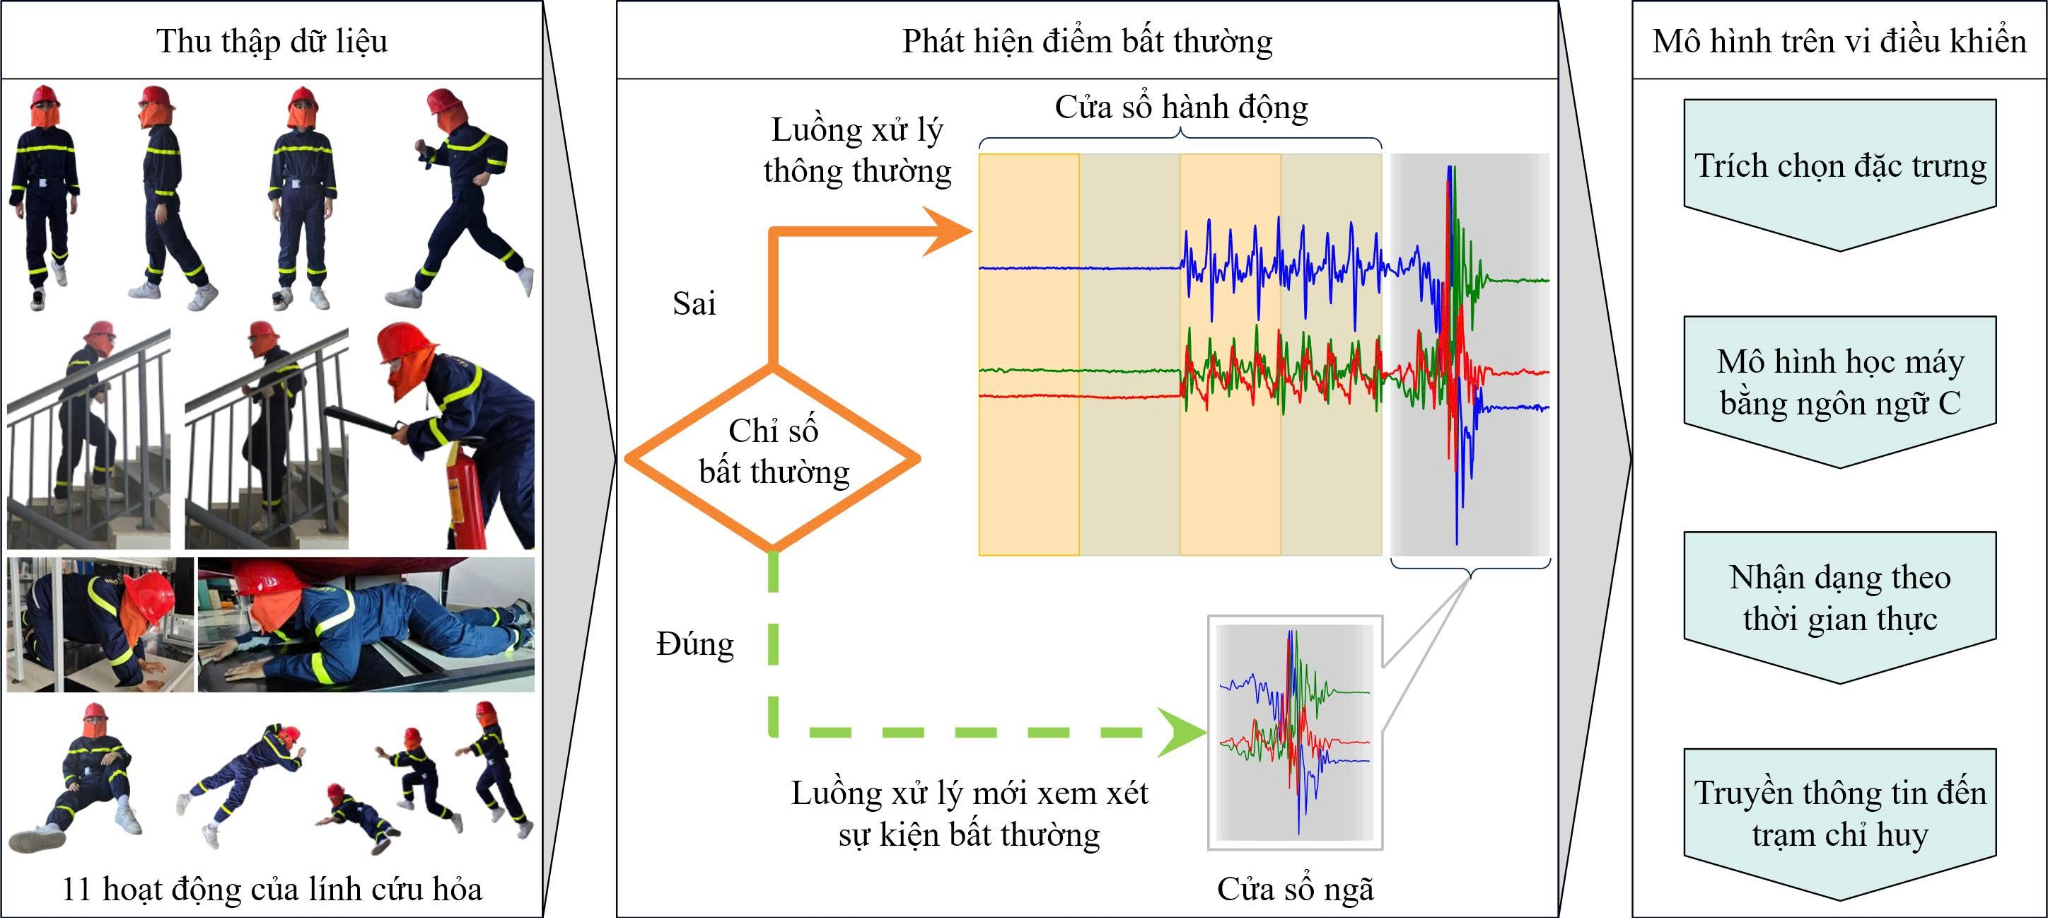
\includegraphics[width=\linewidth,height=.46\textheight,keepaspectratio]{assets/har-abnormal-detection.png}
\caption{Minh họa quy trình thu thập hoạt động, nhận biết cửa sổ tín hiệu bất thường và nhận dạng hành động tại biên}
\label{fig:har-quy-trinh-minh-hoa}
\end{figure}

Cụ thể, tín hiệu gia tốc ba trục từ các hoạt động được phân đoạn thành cửa sổ quan sát trước khi tính 13 đặc trưng miền thời gian như cấu hình mô hình đã nêu. Nhánh quan sát \textit{chỉ số bất thường} trong hình nhằm làm nổi bật các biến động mạnh, chẳng hạn cửa sổ chứa sự kiện ngã, để ưu tiên xem xét riêng; chỉ số này không được đồng nhất với xác suất nhận dạng lớp \emph{ngã} của Random Forest. Sau khi suy luận, kết quả trạng thái được đóng gói để chuyển tiếp theo tuyến BLE--RF--Gateway đã mô tả, không phát MQTT trực tiếp từ ESP32 trên chặng RF. Việc xác nhận ngã và đánh giá cảnh báo giả vẫn phải được kiểm thử độc lập.


Trong quá trình vận hành, cần phân biệt rõ chu kỳ lấy mẫu cảm biến (20 ms tương ứng với tần số 50 Hz) và chu kỳ xuất kết quả nhận dạng của mô hình. Nếu sử dụng các cửa sổ trượt không chồng lấp, kết quả phân loại mới chỉ được cập nhật sau mỗi 3 giây. Gọi $H$ là bước dịch cửa sổ (tính theo số mẫu), chu kỳ cập nhật kết quả sẽ là $H/f_s$. Hệ thống có thể áp dụng phương án chồng lấp 50\% ($H=75$ mẫu) để rút ngắn chu kỳ cập nhật xuống còn 1,5 giây; tuy nhiên cấu hình này cần được đo kiểm thực tế về mức tải CPU và tiêu thụ năng lượng trước khi áp dụng cố định vào mã nguồn.

Tập nhãn mục tiêu trong thiết kế hệ thống bao gồm 11 trạng thái vận động đặc thù: đứng, đi bộ, chạy, ngồi, nằm, đi khom, bò, trườn, ngã, lên cầu thang và xuống cầu thang. Trong đó, hai hành động di chuyển lên và xuống cầu thang được tách thành hai lớp riêng biệt. Bảng ánh xạ giữa mã số nguyên đầu ra của mô hình và tên hành động tương ứng phải được quản lý đồng bộ theo từng phiên bản tệp mô hình biên dịch nhằm tránh gán sai ngữ nghĩa trên giao diện hiển thị.

\subsection{Quy trình tiền xử lý tín hiệu và trích chọn đặc trưng}
Để đảm bảo tính nhất quán toán học, chuỗi dữ liệu gia tốc đưa vào suy luận trên ESP32 phải tuân thủ chính xác đơn vị vật lý, dải đo, chiều trục tọa độ và bộ lọc tiền xử lý như trong giai đoạn huấn luyện mô hình. Khi xảy ra lỗi đọc bus giao tiếp hoặc mất mẫu cục bộ, thuật toán tuyệt đối không tự động điền giá trị 0 vào chuỗi tín hiệu vì thao tác này sẽ tạo ra xung biến thiên giả tạo. Các cửa sổ không thu thập đủ số mẫu quy định sẽ được gắn cờ báo lỗi và loại bỏ khỏi luồng suy luận.

Cấu hình véc-tơ đặc trưng đầu vào gồm 13 thành phần trên miền thời gian được tổ chức từ hai nhóm chính: nhóm thứ nhất gồm giá trị trung bình, độ lệch chuẩn và khoảng biến thiên biên độ tính riêng trên từng trục $x, y, z$ (tạo thành 9 đặc trưng); nhóm thứ hai gồm diện tích biên độ tín hiệu (SMA), năng lượng trung bình, giá trị trung bình độ lớn gia tốc và độ lệch chuẩn độ lớn gia tốc tổng hợp (tạo thành 4 đặc trưng). Thứ tự sắp xếp các phần tử trong mảng đặc trưng trên mã nguồn C/C++ phải khớp tuyệt đối với thứ tự các cột đặc trưng khi huấn luyện mô hình trên Python.

Với một chuỗi tín hiệu thành phần $u_i$ gồm $N$ mẫu trong một cửa sổ quan sát, các đại lượng thống kê cơ sở được tính toán theo công thức:
\begin{align}
\bar u&=\frac{1}{N}\sum_{i=1}^{N}u_i, &
\sigma_u&=\sqrt{\frac{1}{N}\sum_{i=1}^{N}(u_i-\bar u)^2},\\
r_u&=\max_i(u_i)-\min_i(u_i), &
\mathrm{SMA}&=\frac{1}{N}\sum_{i=1}^{N}(|a_{x,i}|+|a_{y,i}|+|a_{z,i}|).
\end{align}
Toàn bộ các biểu thức toán học, bao gồm cả quy ước mẫu số $N$ hay $N-1$ trong công thức tính độ lệch chuẩn, đều phải được đồng bộ giữa kịch bản huấn luyện và hàm tính toán nhúng. Trường hợp mô hình có sử dụng bước chuẩn hóa đặc trưng (scaling), các hằng số trung bình và độ lệch chuẩn của tập huấn luyện phải được trích xuất cứng vào mã nguồn vi điều khiển, không tính toán lại theo từng cửa sổ kiểm thử đơn lẻ.

\subsection{Cơ chế xử lý và xác nhận sự kiện té ngã}
Do té ngã là sự kiện khẩn cấp diễn ra rất nhanh, việc kết luận trạng thái ngã cần được xem xét kết hợp với chuỗi hành động liền trước và liền sau thời điểm va chạm, cùng mức độ tin cậy của bộ phân loại. Việc chỉ sử dụng một cửa sổ trượt cố định kích thước dài có thể gây trễ cảnh báo hoặc làm nhầm lẫn giữa thao tác chuyển tư thế nhanh (như cúi gập người, nằm xuống) với sự kiện ngã thực sự. Do đó, luồng cảnh báo trên giao diện được thiết kế đi kèm cơ chế xác nhận trạng thái bất động tiếp diễn sau va chạm để người chỉ huy có thêm cơ sở kiểm tra.

Về mặt phần cứng mở rộng, việc trang bị thêm nút bấm khẩn cấp (SOS) vật lý và còi báo động tại chỗ trên thiết bị đeo là giải pháp bổ trợ thiết thực, bởi không phải mọi sự cố nguy hiểm tại hiện trường đều biểu hiện qua tín hiệu té ngã. Các tính năng an toàn phần cứng này cần được kiểm thử độc lập với mô hình học máy. Báo cáo phân định rõ kết quả nhận diện nhãn ``ngã'' của thuật toán phân lớp với một hệ thống cảnh báo sinh tồn hoàn chỉnh đạt chuẩn công nghiệp.

\section{Thiết kế thuật toán định hướng và định vị tương đối PDR}\label{sec:pdr}
\subsection{Quy ước hệ trục tọa độ và góc phương vị}
Hệ thống định vị trong nhà sử dụng mặt phẳng tọa độ Đề-các hai chiều với trục $x$ hướng về phía Đông và trục $y$ hướng về phía Bắc. Góc phương vị $\psi$ được quy ước bằng $0^\circ$ tại hướng Bắc và tăng dần theo chiều kim đồng hồ. Trước khi đưa vào thuật toán định vị, các véc-tơ đo lường từ cảm biến được phép biến đổi ma trận từ hệ trục tọa độ nội tại của bo mạch GY-85 sang hệ trục gắn với cơ thể người đeo. Trường hợp trục dọc của mặt bằng tòa nhà lệch một góc so với hướng Bắc từ trường, hệ thống sẽ lưu thêm tham số góc lệch nền $\psi_0$ tại thời điểm khởi tạo để xoay quỹ đạo khớp với bản đồ hiển thị.

Quy ước chia 8 vùng hướng (Bắc, Đông Bắc, Đông, Đông Nam, Nam, Tây Nam, Tây, Tây Bắc), trong đó hướng Bắc bao phủ miền $[337{,}5^\circ,360^\circ)\cup[0^\circ,22{,}5^\circ)$ và các hướng tiếp theo cách đều mỗi cung $45^\circ$, chỉ được sử dụng nhằm mục đích hiển thị trực quan trên giao diện người dùng. Bên dưới tầng tính toán, thuật toán cập nhật tọa độ PDR luôn sử dụng giá trị góc phương vị liên tục để tránh sai số lượng tử hóa. Mọi giá trị góc tính bằng độ đều được quy đổi sang đơn vị radian trước khi đưa vào các hàm lượng giác trong thư viện toán học của vi điều khiển.

\subsection{Hiệu chuẩn cảm biến và thuật toán lọc hợp nhất định hướng}
Quy trình hiệu chuẩn con quay hồi chuyển được thực hiện ngay khi khởi động bằng cách xác nhận một khoảng thời gian thiết bị đứng yên hoàn toàn để ước lượng độ lệch điểm không (bias) ban đầu, đồng thời theo dõi sự biến thiên của tham số này theo nhiệt độ. Đối với cảm biến gia tốc, hệ thống kiểm tra sai số lệch trục và hệ số tỷ lệ độ nhạy. Đối với từ kế, phép hiệu chuẩn khử nhiễu từ trường tĩnh được biểu diễn qua phương trình ma trận:
\begin{equation}
\boldsymbol m_c=\boldsymbol A(\boldsymbol m_{raw}-\boldsymbol b_m),
\end{equation}
trong đó véc-tơ $\boldsymbol b_m$ bù sai số từ cứng (hard-iron) do các nguồn từ cố định trên mạch gây ra, và ma trận $\boldsymbol A$ bù biến dạng từ mềm (soft-iron) do cấu trúc vật liệu sắt từ xung quanh. Cơ sở lý thuyết về hai dạng nhiễu từ trường và thuật toán hiệu chuẩn elipsoid được tham chiếu từ tài liệu kỹ thuật AN4246 của NXP~\cite{magcal}.

Sau bước hiệu chuẩn, véc-tơ từ trường bắt buộc phải được bù góc nghiêng (roll và pitch) trước khi tính toán góc phương vị; việc áp dụng trực tiếp hàm lượng giác $\operatorname{atan2}$ trên hai trục mặt phẳng ngang mà bỏ qua độ nghiêng của thắt lưng sẽ gây ra sai số hướng rất lớn khi người lính cúi hoặc nghiêng người~\cite{compass}. Ngoài ra, khi người dùng chạy hoặc vận động mạnh, gia tốc tổng hợp đo được chứa cả thành phần gia tốc quán tính chuyển động chứ không chỉ riêng gia tốc trọng trường. Vì vậy, thuật toán lọc hợp nhất phải kiểm tra điều kiện ngưỡng độ lớn gia tốc và từ trường trước khi cập nhật, tuyệt đối không đưa mọi mẫu đo bị nhiễu động học vào bộ lọc với cùng một trọng số tin cậy.

Để phân tích sự tiến triển của góc phương vị $\psi_k$ và độ trôi điểm không $b_k$ của con quay hồi chuyển theo chu kỳ lấy mẫu $\Delta t$, mô hình trạng thái tuyến tính rút gọn được biểu diễn dưới dạng:
\begin{equation}
\begin{bmatrix}\psi_{k+1}\\b_{k+1}\end{bmatrix}
=\begin{bmatrix}1&-\Delta t\\0&1\end{bmatrix}
\begin{bmatrix}\psi_k\\b_k\end{bmatrix}
+\begin{bmatrix}\Delta t\\0\end{bmatrix}\omega_{\psi,k}+\boldsymbol w_k,
\end{equation}
trong đó $\omega_{\psi,k}$ là vận tốc góc quay quanh trục thẳng đứng sau khi đã chiếu theo tư thế nghiêng của thiết bị (không đồng nhất hoàn toàn với giá trị đọc thô trên trục $z$ của con quay hồi chuyển ở mọi tư thế), và $\boldsymbol w_k$ là nhiễu quá trình. Phép đo góc hướng từ từ kế chỉ được dùng để hiệu chỉnh trạng thái khi vượt qua bước kiểm tra chất lượng từ trường. Đặc biệt, sai lệch góc đổi mới (innovation) trong bộ lọc luôn được chuẩn hóa về miền đối xứng $[-\pi, \pi]$ nhằm ngăn ngừa hiện tượng nhảy vọt giá trị khi góc quay đi qua ranh giới $0^\circ/360^\circ$.

\subsection{Thuật toán phát hiện bước chân và cập nhật tọa độ tương đối}
Để phát hiện sự kiện bước chân từ vùng thắt lưng, hệ thống tính toán độ lớn gia tốc tổng hợp trên cả ba trục tại thời điểm lấy mẫu thứ $k$ theo công thức:
\begin{equation}
a_k=\sqrt{a_{x,k}^2+a_{y,k}^2+a_{z,k}^2}.
\end{equation}
Chuỗi tín hiệu độ lớn gia tốc sau đó được đưa qua bộ lọc thông thấp để loại bỏ nhiễu tần số cao, kết hợp thuật toán dò tìm cực đại cục bộ có ràng buộc ngưỡng biên độ tối thiểu và khoảng cách thời gian tối thiểu giữa hai bước chân liên tiếp. Các tham số ngưỡng này cần được khảo sát thực nghiệm khi thay đổi tốc độ di chuyển và vị trí gá lắp. Khi mô hình nhận dạng hoạt động ghi nhận người lính chuyển sang tư thế bò, trườn hoặc leo trèo, hệ thống không tiếp tục áp dụng bộ đếm bước đi bộ thông thường.

Tại mỗi thời điểm xác nhận một bước chân hợp lệ thứ $k$ với chiều dài sải bước $\ell_k$ và góc phương vị tức thời $\psi_k$, tọa độ vị trí tương đối $(x_k, y_k)$ và tổng quãng đường di chuyển $D_k$ được cập nhật đệ quy theo hệ phương trình (Hình~\ref{fig:pdr}):
\begin{align}
x_k&=x_{k-1}+\ell_k\sin\psi_k,\\
y_k&=y_{k-1}+\ell_k\cos\psi_k,\\
D_k&=D_{k-1}+\ell_k.
\end{align}
Trong hệ phương trình trên, biến tổng quãng đường $D_k$ chỉ phục vụ mục đích thống kê hành trình, tuyệt đối không lấy $D_k$ cộng dồn vào công thức tính tọa độ ở mỗi bước. Tham số chiều dài bước $\ell_k$ cần được hiệu chuẩn theo thể trạng người dùng hoặc ước lượng thích nghi theo nhịp bước. Đồng thời, thuật toán tách biệt rõ thao tác xoay người tại chỗ (chỉ làm biến thiên góc $\psi_k$) với sự kiện bước chân tịnh tiến nhằm tránh tạo ra các bước dịch chuyển giả trên bản đồ.

\Diagram{pdr}{Lưu đồ thuật toán định vị quán tính PDR thực thi trên thiết bị đeo}{fig:pdr}

\subsection{Phương pháp ước tính biến thiên độ cao từ áp suất khí quyển}
Cảm biến áp suất BMP580 cung cấp dữ liệu đầu vào để hệ thống theo dõi sự dịch chuyển tương đối theo phương thẳng đứng giữa các tầng lầu. Theo mô hình khí quyển đẳng nhiệt tiêu chuẩn, độ chênh lệch độ cao $\Delta h$ so với mốc khởi tạo được ước lượng theo công thức khí áp:
\begin{equation}
\Delta h\approx-\frac{R_dT}{g}\ln\!\left(\frac{p}{p_0}\right),
\end{equation}
trong đó $R_d$ là hằng số khí riêng của không khí khô, $g$ là gia tốc trọng trường, $T$ là nhiệt độ tuyệt đối tính theo thang Kelvin, $p$ là áp suất hiện tại và $p_0$ là áp suất tham chiếu tại tầng xuất phát. Trong thực tế tác nghiệp bên trong tòa nhà, phép đo áp suất chịu ảnh hưởng nhiễu rất lớn từ điều kiện thời tiết, luồng gió lùa, hệ thống quạt tăng áp cầu thang và độ trễ thông khí của vỏ thiết bị. Do đó, hệ thống cần chốt lại áp suất gốc $p_0$ ngay trước khi vào công trình, kết hợp theo dõi xu hướng biến thiên áp suất cùng trạng thái leo cầu thang từ mô hình HAR để phân loại tầng.

\section{Quản lý hệ thống, bảo mật thông tin và phương án dự phòng}
Về mặt quản trị vận hành, toàn bộ thiết bị trong mạng được định danh và theo dõi đồng bộ theo mã phần cứng, mã phiên nhiệm vụ, phiên bản chương trình nhúng (firmware), bộ tham số hiệu chuẩn và dấu thời gian của gói tin cuối cùng. Mỗi khi thay thế mô-đun cảm biến hoặc thay đổi vị trí gá lắp trên trang phục, hệ thống bắt buộc phải thực hiện lại quy trình hiệu chuẩn và kiểm tra lại độ tương thích của mô hình nhận dạng. Khi phát sinh lỗi phần cứng hoặc đứt kết nối, trạm Gateway sẽ ghi nhận mã lỗi cụ thể và đẩy trạng thái cảnh báo kỹ thuật lên giao diện; hệ thống phân biệt rõ ràng giữa cảnh báo lỗi kỹ thuật thiết bị với cảnh báo nguy hiểm sinh tồn từ dữ liệu cảm biến hợp lệ.

Về mặt an toàn thông tin, kết nối mạng IP từ trạm Gateway tới MQTT Broker cần được thiết lập cơ chế xác thực tài khoản, kiểm tra chứng chỉ số khi sử dụng mã hóa TLS và phân quyền truy cập chủ đề (ACL) chặt chẽ theo từng vai trò thiết bị. Các thông tin nhạy cảm như cấu hình SIM, khóa xác thực và mật khẩu máy chủ được lưu trữ bảo mật trong tệp cấu hình hệ thống, tuyệt đối không gắn cứng vào khung bản tin truyền dẫn hay mã nguồn công khai. Do trường kiểm tra CRC 2 byte trong khung tin RF chỉ có tác dụng phát hiện lỗi bit đường truyền chứ không chống được tấn công giả mạo hoặc phát lại gói tin, kênh truyền vô tuyến cục bộ cần được bổ sung thêm cơ chế mã hóa nhẹ khi nâng cấp lên phiên bản thực địa.

Để đảm bảo tính sẵn sàng cao trong điều kiện khẩn cấp, hệ thống thiết lập đồng bộ các cơ chế dự phòng lỗi. Các giải pháp bao gồm: lưu đệm dữ liệu trên thẻ nhớ Gateway khi mất sóng 4G, giới hạn số lần phát lại trên kênh RF để tránh nghẽn mạng, cấu hình dịch vụ tự động khởi động lại tiến trình (watchdog) khi treo phần mềm, trang bị nguồn pin dự phòng và hiển thị cảnh báo trực quan khi dữ liệu quá hạn. Toàn bộ các tính năng dự phòng này đều được đưa vào danh mục bắt buộc phải kiểm thử bằng kịch bản giả lập lỗi thực tế tại Chương 3, không chỉ dừng lại ở việc mô tả trên sơ đồ kiến trúc.

\section{Kết luận chương}
Chương 2 đã trình bày chi tiết thiết kế kiến trúc tổng thể của hệ thống từ cụm thiết bị đeo tại thắt lưng và mũ bảo hộ đến trạm chuyển tiếp Gateway sử dụng Raspberry Pi 3 Model B kết hợp mô-đun SIM 4G. Cấu trúc khung bản tin nhị phân 44 byte, cơ chế quản lý hàng đợi chống trùng lặp và quy trình xử lý tại biên trên vi điều khiển ESP32 đã được chuẩn hóa đồng bộ. Trong đó, phân hệ nhận dạng hoạt động được thiết lập với mô hình Rừng ngẫu nhiên cùng quy trình trích xuất 13 đặc trưng miền thời gian nhất quán; phân hệ định vị tương đối PDR được xây dựng chặt chẽ từ khâu quy ước hệ trục tọa độ, hiệu chuẩn bù nghiêng từ kế đến công thức cập nhật vị trí theo từng bước chân. Toàn bộ các thông số thiết kế này là cơ sở kỹ thuật trực tiếp để xây dựng kịch bản kiểm thử định lượng và phân tích đánh giá hệ thống tại các chương tiếp theo.